\subsection{Earthframe and bodyframe}\label{chapter_EQUATIONS_OF_MOTION}

This - and the following - chapter discusses the behaviour of a quadrocopter. To achieve a better understanding, graphics with a simplified model of the quadrocopter are used. This model consists of a middle cross, and the four rotors with arrows, showing the direction of rotation. The rotor at the front is marked in yellow.
Placing a coordinate system on the cross of the quadrocopter, the x-axis points to the front, the y-axis to the left and the z-axis points upwards. This coordinate system is called the bodyframe and is shown in red in the picture below.

\begin{figure}[htbp]
	\centering
		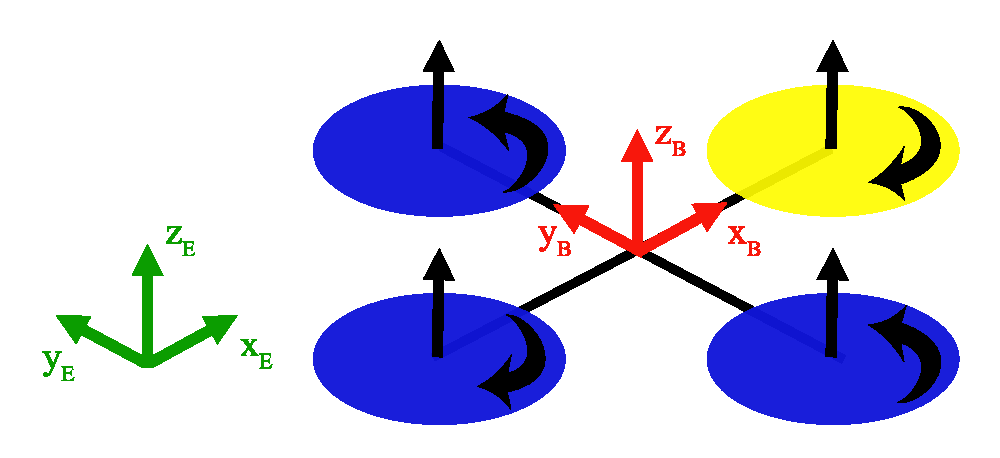
\includegraphics[width=0.7\textwidth]{03_Grafiken/EFrameBFrame.pdf}
	\caption{Earthframe (green) and bodyframe (red)}
	\label{fig:EFrameBFrame}
\end{figure}

The green coordinate system is called the earthframe. This coordinate system is fix and independent of the movement of the quadrocopter. It describes the position of the copter, whereat the copter is interpreted as a point. It also describes the associated velocities and accelerations in direction of x, y and z of the earthframe.
So the earthframe does not contain information about the attitude of the quadrocopter. This information is held by the bodyframe, that includes the angles of the coordinate system in relation to the earthframe, as well as the angular rates and -accelerations. It also holds information about the movement in direction of the axis of the bodyframe coordinate system, wherat the movement in direction of x and y of the bodyframe is a side effect of gravity, while movement in direction of z can be controlled directly.

So, 'sitting' on the bodyframe of the quadrocopter, it is not possible to know the position in space, but it is possible to know the deviation from horizontal in degrees as well as the vertical speed of spinning. Sitting on the eartframe, it is possible to see where the quadrocopter is, and how fast it is moving, but it is impossible to know if it is perhaps flying upside down.

Though these two frames hold different information, there is a mathematical association in between. This is explained in a simple two-dimensional example below.

\begin{figure}[htbp]
	\centering
		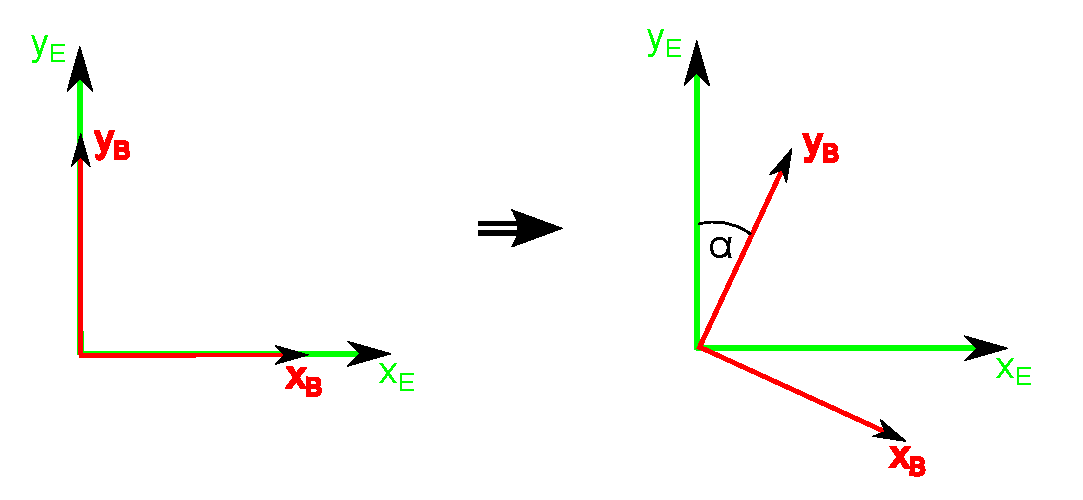
\includegraphics[width=1.0\textwidth]{03_Grafiken/2DFrames.pdf}
	\caption{Association between earthframe and bodyframe}
	\label{fig:2DFrames}
\end{figure}

In the left picture, the two-dimensional bodyframe is congruent with the earthframe. If there is a constant velocity $v_{yB}$ in direction of $y_B$:
\begin{center}
	$v_{yE} = v_{yB}$
\end{center}
Furthermore 
\begin{center}
	$v_{xE} = 0$ 
\end{center}
In the second picture, the bodyframe is rotated a constant angle alpha; $v_{yB}$ is still constant. Now it is: 
\begin{center}
$v_{yE} = cos(\alpha)*v_{yB}$
\end{center}
and 
\begin{center}
$v_{xE} = sin(\alpha)*v_{yB}$
\end{center}
So it is possible to transform coordinates of the bodyframe into coordinates of the earthframe and vice versa.